\documentclass{article}
\usepackage[margin=1in]{geometry}
\usepackage{microtype}
\usepackage{setspace}
\usepackage{amsmath}
\usepackage{parskip}
\usepackage{amssymb}
\usepackage{graphicx}

\graphicspath{{../public/}}

\parskip=4ex
\date{}
\author{}

\usepackage{tikz-3dplot}
\title{11.1 Functions of Several Variables}

\begin{document}
    \maketitle
    \textbf{Definition}\\
    A function $ f $ of two variables is a rule that assigns to each ordered pair of real numbers $ (x,y) $ in a set $ D $ a unique real number denoted by $ f(x,y) $. The set $ D $ is the domain of $ f $ and its range is the set of values $ f $ takes on, that is
    \[
      \{ f(x,y) | (x,y) \in D \} 
    \]

    At often times, $ z=f(x,y) $ is written to make explicit the value taken on by $ f $ at the general point $ (x,y) $. So $ x ~\&~ y $ are independent variables and $ z $ is the dependent variable.

    A function of two variables is just a function whose domain is a subset of $ \mathbb{R}^{2}  $ and whose range is a subset of $ \mathbb{R} $. If a function $ f $ is given by a formula and no domain is specified, then the domain of $ f $ is the set $ \{ (x,y)|x,y \in \mathbb{R} \} $.

  \textbf{Ex 1}\\
  Find the domains of the following functions and evaluate $ f(3,2) $.\\
  A) $ f(x,y)=\frac{\sqrt{x+y+1}}{x-1}$\\
  B) $ f(x,y) =x\ln(y^{2}-x) $ 

  \textbf{Ex 1A}
  \[
      \begin{gathered}
      f(x,y)=\frac{\sqrt{x+y+1}}{x-1}\\
      ~\\
      f(3,2)=\frac{\sqrt{6}}{2}\\
      ~\\ 
      D=\{ (x,y) | x+y+1\ge 0,x \neq 1\}
      \end{gathered}
  \]

  \textbf{Ex 1B}
  \[
      \begin{gathered}
      f(x,y)=x\ln(y^{2}-x)\\
      ~\\
      f(3,2)=0\\
      ~\\
      D=\{ (x,y)|y^{2}-x>0\}
      \end{gathered}
  \]

  \textbf{Ex 2}\\
  Find the domain and range of $ g(x,y)=\sqrt{9-x^{2}-y^{2}}$.
  \[
      D=\{ (x,y)|9-x^{2}-y^{2}\ge0\} \qquad R=\{ z|z=\sqrt{9-x^{2} -y^{2} },(x,y) \in D \}
  \]

  \textbf{Graphs}\\
  If $ f  $ is a function of two variables with domain $ D $, then the graph of $ f $ is the set of all points $ (x,y,z) $ in $ \mathbb{R}^{3} $ such that $ z=f(x,y) ~\&~ (x,y$ is in $ D $. 

  Just as the graph of a single variable function $ f $ is a curve $ C $ with the equation $ y=f(x) $, the graph of a double variable function $ f $ is a surface $ S $ with equation $ z=f(x,y) $. The graph $ S $ of $ f $ can be visualizd as lying directly above or below its domain $ D $ in the $ xy $ plane.
  \begin{center}
    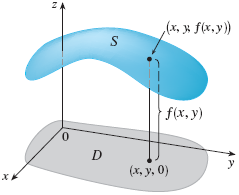
\includegraphics[width=6cm]{11_1_1}
  \end{center}

  \textbf{Ex 3}\\
  Sketch the graph of the function $ f(x,y)=6-3x-2y $
  \[
    \begin{gathered}
    z=f(x,y)=6-3x-2y \to z=6-3x-2y\\
    3x+2y+z=6 \qquad \text{equation for a plane}\\
    ~\\
    XYZ \text{ Intercepts}\\
    x=2,y=3,z=6
    \end{gathered}
  \]
  \begin{center}
    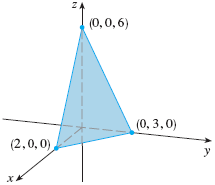
\includegraphics[width=6cm]{11_1_2}
  \end{center}

  \textbf{Level Curves}\\
  The level curves of a function $ f $ of two variables are the curves with equations $ f(x,y)=k $, where $ k $ is a constant (in the range of $ f $ ).

  A level curve $ f(x,y) =k$ is the set of all points in the domain of $ f $ at which $ f $ takes on a given value $ k $. Meaning that it shows where the graph of $ f $ has height $ k $. 

  \textbf{Applications of Level Curves}\\
  An example of level curves being applied can be seen in topographic m aps of mountainous regions. The level curves are curves of constant elevation above sea level. Another one would be the temperature function. In which the level curves are known as isothermals and join locations with the same temperatures as shwon below.
  \begin{center}
    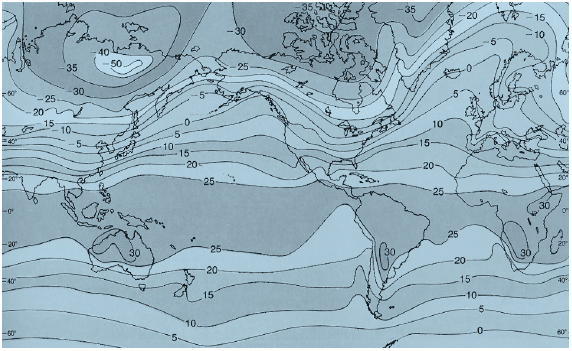
\includegraphics[width=12cm]{11_1_3}
  \end{center}

  \textbf{Ex 6}\\
  A countour map for a function $ f $ is shown below. Use it to estimate the values of $ f(1,3) ~\&~ f(4,5)$.
  \begin{center}
    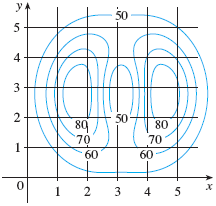
\includegraphics[width=7cm]{11_1_4}
  \end{center}
  \[
    f(1,3) \approx 73 \qquad f(4,5) \approx 56
  \]

  \textbf{Ex 7}\\
  Sketch the level curves of the function $ f(x,y) =6-3x-2y$ for the values $ k=-6,0,6,12 $
  \[
    \begin{gathered}
      6-3x-2y=k \to 3x+2y+(k-6)=0\\
      ~\\
      k=-6,0,6,12\\
      3x+2y-12=0 \qquad 3x+2y-6=0 \qquad 3x+2y=0 \qquad 3x+2y+6=0
    \end{gathered}
  \]
  \begin{center}
    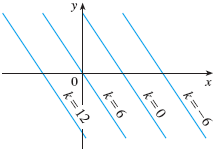
\includegraphics[width=5cm]{11_1_5}
  \end{center}
 
  \textbf{Functions of Three or More Variables}\\
  A function of three variables, $ f $, is a rule that assigns to each ordered triple $ (x,y,z) $ in a domain $ D \subset \mathbb{R}^{3} $. To exemplify, the temperature $ T $ at a point on Earth's surface depends on the longitude, latitude, and time or respectively $ x,y,~\&~ t $. So the temperature $ T $ is a function of those variables $ x,y ~\&~ t $.
  \[
    T=f(x,y,t)
  \]
 
  \textbf{Ex 10}\\
  Find the domain of $ f $ if $ f(x,yz=ln(z-y)+xy\sin{z}) $.
  \[
   D=\{ (x,y,z) \in \mathbb{R}^{3} | z-y>0  \} 
   \]
\end{document}
